% Capitulo 2

\chapter{Estado del Arte} % Main chapter title

\label{EstadoDelArte} % For referencing the chapter elsewhere, use \ref{Chapter1} 

\lhead{Capítulo 2 \emph{Estado del Arte}} % This is for the header on each page - perhaps a shortened title

%----------------------------------------------------------------------------------------

Existen dos clases de aplicaciones que se analizaron: aplicaciones con localización en interiores y otras que brindan información sobre aeropuertos. Las Tablas \ref{tab:appsInteriores} y \ref{tab:appsViajes} muestran estas aplicaciones.

\definecolor{blanco}{RGB}{255,255,255}

\begin{table}
	\begin{center}
		\begin{tabular}{|p{1.8cm}|p{4.5cm}|p{1.05cm}|p{2.5cm}|p{2.5cm}|}
			\hline \rowcolor[RGB]{0,102,204} 
			\textcolor{blanco}{\bf Aplicación} &
				\textcolor{blanco}{\bf Descripción} &
					\textcolor{blanco}{\bf Precio} &
						\textcolor{blanco}{\bf Plataforma(s)} &
							\textcolor{blanco}{\bf Logotipo} \\
			\hline \rowcolor[RGB]{224,224,224} 
			\multirow{8}{0cm}{Crux} &
				Aplicación móvil que permite conocer la ubicación en interiores. Ofrece herramientas para potenciar las ventas, las visitas, la fidelidad de los clientes, la experiencia de compra y su grado de satisfacción. \cite{crux} &
					\multirow{8}{0cm}{Gratis} &
						\multirow{8}{0cm}{Android} &
							\multirow{7}{0cm}{\raisebox{-\totalheight}{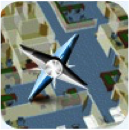
\includegraphics[width=25mm, height=25mm]{Figuras/crux.png}}} \\
      		\hline 
      		\multirow{8}{0cm}{Meridian} &
      			Guía a los viajeros paso a paso hacia el lugar que deseen visitar dentro del aeropuerto. Integra bases de datos de las tiendas en el aeropuerto, horarios de vuelos y cuentas de redes sociales. \cite{meridian} &
      				\multirow{8}{0cm}{Gratis} &
      					\multirow{8}{0cm}{iOS y Android} &
      						\multirow{7}{0cm}{\raisebox{-\totalheight}{
\includegraphics[width=25mm, height=25mm]{Figuras/meridian.png}}} \\
      		\hline 
		\end{tabular}
	\end{center}
	\caption[Aplicaciones para Localización en Interiores]{Aplicaciones para localización en Interiores} 
	\label{tab:appsInteriores}
\end{table}


\begin{table}
	\begin{center}
		\begin{tabular}{|p{1.8cm}|p{4.5cm}|p{1.05cm}|p{2.5cm}|p{2.5cm}|}
			\hline \rowcolor[RGB]{76,153,0}
			\textcolor{blanco}{\bf Aplicación} &
				\textcolor{blanco}{\bf Descripción} &
					\textcolor{blanco}{\bf Precio} &
						\textcolor{blanco}{\bf Plataforma(s)} &
							\textcolor{blanco}{\bf Logotipo} \\
			\hline \rowcolor[RGB]{224,224,224} 
			\multirow{12}{0cm}{GateGuru} &
				Recibe datos de unos 180 aeropuertos ubicados en EE.UU., Canadá, Europa y Asia, de tal forma que da a conocer el estado de vuelos. La aplicación también permite visualizar itinerarios conectándose con Tripit y Kayak. Además de obtener mapas, información sobre el clima y alquileres de coche. \cite{gateguru} &
					\multirow{12}{0cm}{Gratis} &
						\multirow{12}{2.5cm}{iOS, Android y Windows Phone} &
							\multirow{11}{0cm}{\raisebox{-\totalheight}{
\includegraphics[width=25mm, height=25mm]{Figuras/gateGuru.png}}} \\
      		\hline \multirow{11}{0cm}{Kayak} &
      			Es un gran buscador que ahora ha pasado a ser también una aplicación. Con Kayak se pueden comparar ofertas de vuelo, hoteles y alquileres de coches, así como buscar tarifas de equipajes; acceder a los teléfonos de las aerolíneas y a la información de los aeropuertos. \cite{kayak} &
      				\multirow{11}{0cm}{Gratis} &
      					\multirow{11}{2.5cm}{iOS, Android, Windows Phone y Kindle Fire.} &
      						\multirow{10}{0cm}{\raisebox{-\totalheight}{
\includegraphics[width=25mm, height=25mm]{Figuras/kayak.png}}} \\
      		\hline \rowcolor[RGB]{224,224,224} 
      		\multirow{9}{0cm}{Tripit} &
      			Es un organizador de viajes que se puede usar desde el teléfono o la tableta en conexión directa con tripit.com.
Además la aplicación alerta sobre posibles retrasos de vuelos y cuenta con un despertador, muy útil si se viaja temprano. \cite{tripit} &
					\multirow{9}{1.05cm}{\$ 49 anual} &
						\multirow{9}{2.5cm}{iOS, Android, Blackberry y Windows Phone.} &
							\multirow{8}{0cm}{\raisebox{-\totalheight}{
\includegraphics[width=25mm, height=25mm]{Figuras/tripit.png}}} \\
      		\hline
		\end{tabular}
	\end{center}
	\caption[Aplicaciones con Información de Viajes]{Aplicaciones con Información de Viajes} 
	\label{tab:appsViajes}
\end{table}

\newpage
A continuación se muestra una recopilación de las publicaciones que se han desarrollado sobre la localización en interiores.

\begin{table}
	\begin{center}
		\begin{tabular}{|p{4cm}|p{4.5cm}|p{4.5cm}|}
			\hline \rowcolor[RGB]{0,0,0} 
			\textcolor{blanco}{\bf Artículo}	 &
				\textcolor{blanco}{\bf Autores} &
					\textcolor{blanco}{\bf Resumen} \\
			\hline \rowcolor[RGB]{224,224,224} 
			\multirow{8}{4cm}{ILS (Indoor Location Systems) Sistemas de Localización en Interiores} &
				\multirow{8}{4.5cm}{Raúl Sánchez Vítores} &
					Este trabajo presenta los problemas existentes de la localización en interiores para después presentar una clasificación de los sistemas ILS y las distintas soluciones técnicas que se han desarrollado. \cite{ILS} \\
      		\hline \multirow{9}{4cm}{Uso del campo magnético de la tierra para localizar a las personas en interiores} &
      			\multirow{9}{4.5cm}{Carlos Eric Galván Tejada \newline
				Juan Pablo García Vázquez \newline
				Jorge Isaac Galván Tejada} &
      				Este trabajo explica las técnicas que se emplean para localizar en interiores utilizando el campo magnético y menciona las ventajas que se tienen a comparación de otras formas de realizar la localización en interiores. \cite{usoCampoMagnetico} \\
      		\hline 
		\end{tabular}
	\end{center}
	\caption[Publicaciones sobre Localización en Interiores]{Publicaciones sobre Localización en Interiores} 
	\label{tab:publicacionesInteriores}
\end{table}



%----------------------------------------------------------------------------------------